\begin{homeworkProblem}

\textbf{Approximating the Optimal Value Function}

Consider a finite MDP $M=\langle \mS, \A, T, \R, \gamma\rangle$, where $\mS$ is the state space, $\A$ action space, $T$ transition probabilities, $\R$ reward function and $\gamma$ the discount factor. Define $Q^*$ to be the optimal state-action value $Q^*(s, a)=Q_{\pi^*}(s, a)$ where $\pi^*$ is the optimal policy. Assume we have an estimate $\tilde{Q}$ of $Q^*$, and $\tilde{Q}$ is bounded by $L_{\infty}$ norm as follows:
$$\|\tilde{Q}-Q^*\|_{\infty} \leq \epsilon$$
Where $\|x\|_{\infty}=\max\limits_{s, a}|x(s, a)|$. \\
Assume that we are following the greedy policy with respect to $\tilde{Q}, \pi(s)=\argmax\limits_{a \in \A} \tilde{Q}(s, a)$. We want to show that the following holds:
$$V_\pi(s) \geq V^*(s)-\frac{2 \epsilon}{1-\gamma}$$
Where $V_{\pi}(s)$ is the value function of the greedy policy $\pi$ and $V^*(s)=\max\limits_{a \in \A} Q^*(s, a)$ is the optimal value function. This shows that if we compute an approximately optimal state-action value function and then extract the greedy policy for that approximate state-action value function, the resulting policy still does well in the real MDP.

(a) Let $\pi^*$ be the optimal policy, $V^*$ the optimal value function and as defined above $\pi(s)=\argmax\limits_{a \in \A} \tilde{Q}(s, a)$. Show the following bound holds for all states $s \in \mS$.
$$V^*(s)-Q^*(s, \pi(s)) \leq 2 \epsilon$$

(b) Using the results of part 1, prove that $V_\pi(s) \geq V^*(s)-\frac{2\epsilon}{1-\gamma}$. \\
Now we show that this bound is tight. Consider the 2-state MDP illustrated in Figure \ref{fig:approximate}. State $s_1$ has two actions, ``\textit{stay}" self transition with reward 0 and ``\textit{go}" that goes
to state $s_2$ with reward $2\epsilon$. State $s_2$ transitions to itself with reward $2\epsilon$ for every time step afterwards.
\begin{figure}[h]
    \centering
    \vspace{-0.4cm}
    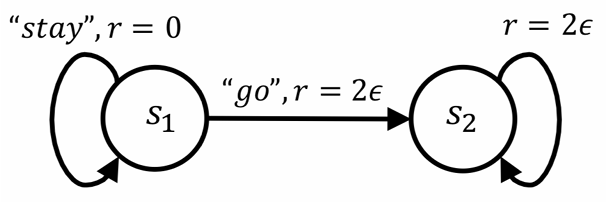
\includegraphics[width=0.5\textwidth]{./figure/approximate.png}
    \vspace{-0.4cm}
    \caption{A 2-state MDP.}
    \vspace{-0.4cm}
    \label{fig:approximate}
\end{figure}

(c) Compute the optimal value function $V^*(s)$ for each state and the optimal stateaction value function $Q^*(s, a)$ for state $s_1$ and each action.

(d) Show that there exists an approximate state-action value function $\tilde{Q}$ with $\epsilon$ error (measured with $L_{\infty}$ norm), such that $V_\pi\left(s_1\right)-V^*\left(s_1\right)=-\frac{2 \epsilon}{1-\gamma}$, where $\pi(s)=$ $\argmax\limits_{a \in \A} \tilde{Q}(s, a)$. (You may need to define a consistent tie break rule)

\solution

(a) Since $\pi(s)$ is the optimal policy for $\tilde{Q}$, thus it has $\tilde{Q}(s, \pi(s)) \geq \tilde{Q}(s, \pi^*(s))$, so
\begin{align*}
V^*(s)-Q^*(s,\pi(s)) &= V^*(s)-\tilde{Q}(s,\pi(s))+\tilde{Q}(s,\pi(s))-Q^*(s,\pi(s)) \\
\text{(Since $\|\tilde{Q}-Q^*\|_{\infty} \leq \epsilon$)}\quad & \leq V^*(s) - \tilde{Q}(s, \pi(s)) + \epsilon \\
\text{(Since $\tilde{Q}(s, \pi(s)) \geq \tilde{Q}(s, \pi^*(s))$)}\quad & \leq V^*(s) - \tilde{Q}(s, \pi^*(s)) + \epsilon \\
&= Q^*(s, \pi^*(s)) - \tilde{Q}(s, \pi^*(s)) + \epsilon \\
\text{(Since $\|\tilde{Q}-Q^*\|_{\infty}\leq \epsilon$)}\quad & \leq 2\epsilon
\end{align*}
So above all, we have proved that $V^*(s) - Q^*(s, \pi(s)) \leq 2\epsilon$.

(b) Using Bellman Exceptation Equation, we have
\begin{align*}
Q^*(s, a) &= \R_s^{a} + \gamma\sum_{s'\in\mS}\mP_{s,s'}^aV^*(s') \\
\tilde{Q}(s, a) &= \R_s^{a} + \gamma\sum_{s'\in\mS}\mP_{s,s'}^aV_{\pi}(s')
\end{align*}
Combining them, we can get that
\begin{align*}
V^*(s) - V_{\pi}(s) &= V^*(s) - Q^*(s, \pi(s)) + Q^*(s, \pi(s)) - V_{\pi}(s) \\
\text{(Conclusion of (a))}\quad &\leq 2\epsilon + Q^*(s, \pi(s)) - Q(s, \pi(s)) \\
&= 2\epsilon + \left(\R_{\pi(s)}^{a} + \gamma\sum_{s'\in\mS}\mP_{\pi(s),s'}^aV^*(s')\right) - \left(\R_{\pi(s)}^{a} + \gamma\sum_{s'\in\mS}\mP_{\pi(s),s'}^aV_{\pi}(s')\right) \\
&= 2\epsilon + \gamma\sum_{s'\in\mS}\mP_{\pi(s),s'}^a\left(V^*(s') - V_{\pi}(s')\right)
\end{align*}
Suppose that the upper bound of $V*(s)-V_{\pi}(s)$ is $U$, i.e. $\forall s \in \mS, V^*(s)-V_{\pi}(s) \leq U$, thus we have:
\begin{align*}
\forall s \in \mS,\quad V^*(s) - V_{\pi}(s) &\leq 2\epsilon + \gamma U \\
\Rightarrow \qquad\qquad\qquad\quad U &\leq 2\epsilon + \gamma U \\
\Rightarrow \qquad\qquad (1-\gamma)U &\leq 2\epsilon \\
\Rightarrow \qquad\qquad\qquad\quad U &\leq \dfrac{2\epsilon}{1-\gamma}
\end{align*}
So above all, we have proved:
$$V^*(s) - V_{\pi}(s)\leq \dfrac{2\epsilon}{1-\gamma} \Rightarrow V_{\pi}(s) \geq V^*(s) - \dfrac{2\epsilon}{1-\gamma}$$

(c) It is obvious that the optimal policy is $\pi_*(s_1)=\text{go}$, from the Bellman Optimility Equation, we have
\begin{align*}
V^*(s_2) &= 2\epsilon + \gamma V^*(s_2) \Rightarrow V^*(s_2) = \frac{2\epsilon}{1-\gamma} \\
V^*(s_1) &= V^{\pi_*}(s_1) = 2\epsilon + \gamma V^*(s_2) \Rightarrow V^*(s_1) = \frac{2\epsilon}{1-\gamma} \\
Q^*(s_1, \text{go}) &= 2\epsilon + \gamma V^*(s_2) \Rightarrow Q^*(s_1, \text{go}) = \frac{2\epsilon}{1-\gamma} \\
Q^*(s_1, \text{stay}) &= 0 + \gamma V^*(s_1) \Rightarrow Q^*(s_1, \text{stay}) = \frac{2\epsilon\gamma}{1-\gamma}
\end{align*}

(d) Since the approximate state-action value function allowed the $\epsilon$ error, and we could observe that the difference between $Q^*(s_1,\text{go})$ and $Q^*(s_1,\text{stay})$ is $\dfrac{2\epsilon}{1-\gamma} - \dfrac{2\epsilon\gamma}{1-\gamma} = 2\epsilon$. Thus we can set $\tilde{Q}$ to be
\begin{align*}
\tilde{Q}(s_1, \text{go}) = Q^*(s_1, \text{go}) - \epsilon &\Rightarrow \tilde{Q}(s_1,\text{go}) = \frac{\epsilon(1+\gamma)}{1-\gamma} \\
\tilde{Q}(s_1, \text{stay}) = Q^*(s_1, \text{stay}) + \epsilon &\Rightarrow \tilde{Q}(s_1,\text{stay}) = \frac{\epsilon(1+\gamma)}{1-\gamma}
\end{align*}
Since the estimated $\tilde{Q}$ for state $s_1$ and its two actions are tie, so we can define the policy for tie: $\pi(\text{stay}|s_1)=1$. Thus $V_{\pi}(s_1)=0 + \gamma V_{\pi}(s_1)\Rightarrow V_{\pi}(s_1)=0$.
Since $V^*(s_1)=\dfrac{2\epsilon}{1-\gamma}$, thus $V_{\pi}(s_1)-V^*(s_1)=-\dfrac{2\epsilon}{1-\gamma}$.

So above all, we have proved that the $V_{\pi}(s)\geq V^*(s)-\dfrac{2\epsilon}{1-\gamma}$ is a tight bound.

\end{homeworkProblem}

\newpage